\section{Généralités}

	Il nous a paru important lors de la réalisation de ce projet
	de mettre au point un code facilement améliorable et surtout
	réutilisable par le spersonnes qui souhaiteraient personnaliser
	le jeu à leur façon.
	
	C'est pourquoi un des points primordial à été tout d'abord de
	rédiger notre code ainsi que notre documentation totallement 
	en Anglais afin qu'une majorité de personne puisse les comprendre.

\section{Client}

	\subsection{Modèles de conception}
	
		\subsubsection{MVC}
		
			Le Modèle-Vue-Contrôleur est une architecture et une méthode de
			conception qui organise l'interface homme-machine (IHM) d'une 
			application logicielle.
			Pour cela il divise l'IHM en un modèle (modèle de données),
			une vue (présentation, interface utilisateur) et un contrôleur
			(gestion des événements, synchronisation), chacun ayant un rôle
			précis dans l'interface.
			
			\begin{center}
				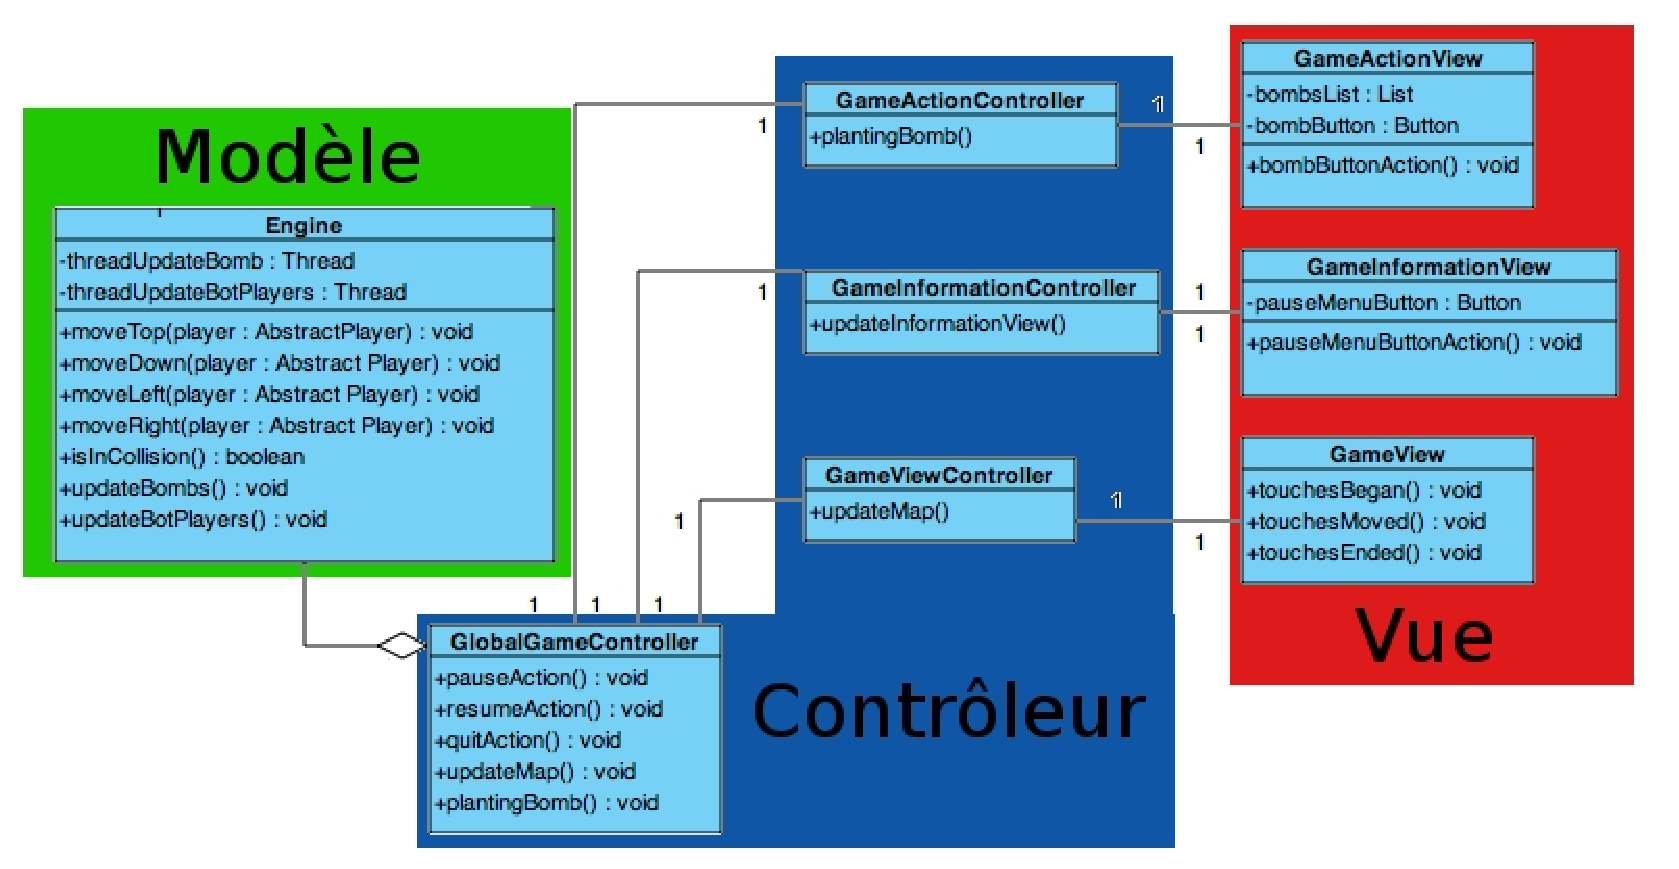
\includegraphics[width=11cm]{./Reutilisabilite/Img/mvc.eps}
			\end{center} 
			
			L'avantage de cette méthode de conception est qu'elle permet la
			modification d'une des parties sans affecter les autres.
			Il serait dans notre cas possible de pouvoir modifier le gameplay,
			l'interface graphique ou encore d'améliorer le moteur du jeu sans pour
			cela devoir s'occuper du reste du code.		
		
		\subsubsection{Design Pattern Décorateur}
		
			\begin{center}
				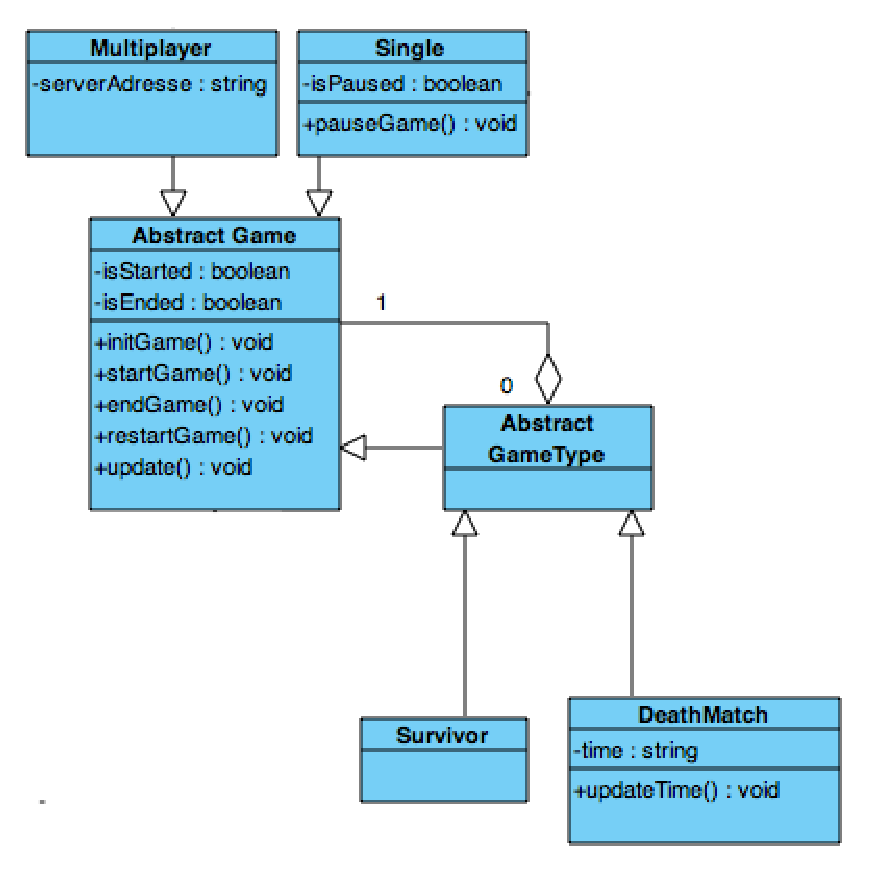
\includegraphics[width=11cm]{./Reutilisabilite/Img/decorateur.eps}
			\end{center} 
		
	\subsection{XML}
	
		Le fait d'avoir utilisé le \gls{xml} permet de pouvoir modifier les diverses caractéristiques de nos
		ressources sans necessiter la moidre modification du code source.
	
		\subsubsection{Internationalisation}
		
			Dans notre jeu nous avons prit en charge le support de l'internationalisation.
			Pour cela nous nous avons dédié à chaque langue un fichier \gls{xml} contenant
			la globalité des mots apparaissants dans notre application.
			Si l'utilisateur souhaite en rajouter une nouvelle langue, il lui suffira d'ajouter
			un fichier \gls{xml} dans le répertoire correspondant à la langue voulu et d'y traduire
			tous les mots présents dans les \gls{xml} des langues déjà existants.
	
		\subsubsection{Personnalisation}
	
			Là aussi l'utilisation du \gls{xml} montre ses avantages lors de la personnalisation
			des diverses ressources mises à disponibilité de l'utilisateur.
			
			Prenons par exemple le code \gls{xml} d'un objet indestructible :
			
			$\,$
		
			\begin{footnotesize}
				\lstset{tabsize=1, frame=shadowbox, rulesepcolor=\color{gray}}
				\lstinputlisting{./Reutilisabilite/code/objects.xml}
			\end{footnotesize}
			
			Si l'on souhaite associer un son à cet objet il suffit d'éditer l'attribut \emph{sound}
			et de rajouter le nom de celui que l'on souhaite.
			Il est en de même pour les différentes caractéristiques de notre objet.		

\section{Serveur}

	\subsection{Servlets}